\section{Raft} \label{sec:raft}

In this section we are not going to present the Raft algorithm, since Ongaro and Ousterhout already did so in their excellent work "In Search of an Understandable Consensus Algorithm" \cite{raft}. Instead, we will discuss the interpretation and implementation we did to adapt it to our own use case.

The algorithm uses three types of nodes, namely leader, follower and candidate, and revolves around three core functionalities: leader election, log replication and overwriting, and cluster membership change. Log compaction is also mentioned, while a byzantine fault tolerant variant is never explored by the original authors.

One last element, fundamental to the functioning of the algorithm, is the \textit{term}: everything happens in a certain term, which divides time logically and increments every election. 

Our Raft class directly extends \textit{simpleXMLRPCServer} from XML-RPC module, as seen at code \ref{code:raft}.

\label{code:raft}
\begin{python} 
class Raft(SimpleXMLRPCServer):
    def __init__(self, 
                 addr: tuple[str, int],
                 allow_none: bool = True,
                 # ...
                 last_index_on_server: list[tuple[int, int]] | None = None
                 ):
        SimpleXMLRPCServer.__init__(self, addr=addr, allow_none=allow_none)
\end{python}

\subsection{Node Types} \label{sec:nodes}

There are three types of node, namely leader, follower and candidate (code \ref{code:nodeModes}). In this section we are going to show their characteristics and similarities. Note that all nodes have a timer: it is randomized for each of them and has been implemented by extending \textit{threading.Timer} \ref{code:loopingTimer}

\label{code:nodeModes}
\begin{python} 
class Raft(SimpleXMLRPCServer):
    class Mode(Enum):
        LEADER = 1
        CANDIDATE = 2
        FOLLOWER = 3
                
    def __init__(self, 
                 # ...
                 mode: Mode = Mode.FOLLOWER,
                 )
\end{python}

\label{code:loopingTimer}
\begin{python} 
class LoopTimer(Timer):
    def __init__(self, interval, function, args=None, kwawrgs=None):
        Timer.__init__(self, interval, function, args, kwawrgs)
        self.was_reset : bool = False
    # ...

class Raft(SimpleXMLRPCServer):
    def __init__(self, 
                 # ...
                 )
        # start timer
        self.timer = LoopTimer(timeout, self.on_timeout)
        self.timer.start()
\end{python}

\subsubsection{Leader Node}

The algorithm revolves around one leader node, whose job is to synchronize all servers' logs to ensure data consistency. It does so by replicating its own log on all followers (the non-leader nodes) by sending new or, if needed, old entries via remote procedure calls. 

To make sure all nodes believe the leader's alive, it sends periodically (every 150-300ms) an empty remote procedure call called \textit{heartbeat}

\subsubsection{Follower Node}

All nodes, except for the leader, are classified as followers. They are not allowed to replicate their own log, and when they receive any request they have to forward them to the leader.

To make sure that the cluster never remains without a leader, every follower have an election timeout (between 150ms and 300ms) which resets every time an RPC from the leader gets received. If it times out, the follower change its state to \textit{candidate}, increment its current term and starts a leader election. 

Followers become candidates in another scenario: whenever they receive an entry from the leader, they compare it with their own last log entry. If either leader's term is smaller, or leader's index is smaller while having the same term, the append is rejected and a new election is started. 

\subsubsection{Candidate Node}

When a follower's election timeout times out, it becomes a candidate and starts an election. It votes for itself and then wait for either of two outcomes: it wins, thus becoming a new leader, or looses (ether another leader gets elected or the old one manifest itself) thus reverting back to being a follower.

\subsection{Log}

As stated, the leader's job is to accept requests (in our specific case they are player inputs) and then forward them to the followers. Let's talk about the structure of the log. 

The log is basically a \textit{list} (or an \textit{array}) of entries, where entry is an element that encapsulates data (like an integer or a string), has an index (unique for each entry) and the term of its creation (figure \ref{fig:logStructure}). We defined entires as Python \textit{Data Classes} \footnote{Data Classes module provides a decorator and functions for automatically adding generated special methods to user-defined classes: \url{https://docs.python.org/3/library/dataclasses.html}} (decorators that simulate C's structures) such as shown in code snippet \ref{code:entry}.

\label{code:entry}
\begin{python} 
@dataclass
class Entry:
    term: int
    index: int
    command: str 
\end{python}

\begin{figure}[h]
  \centering
  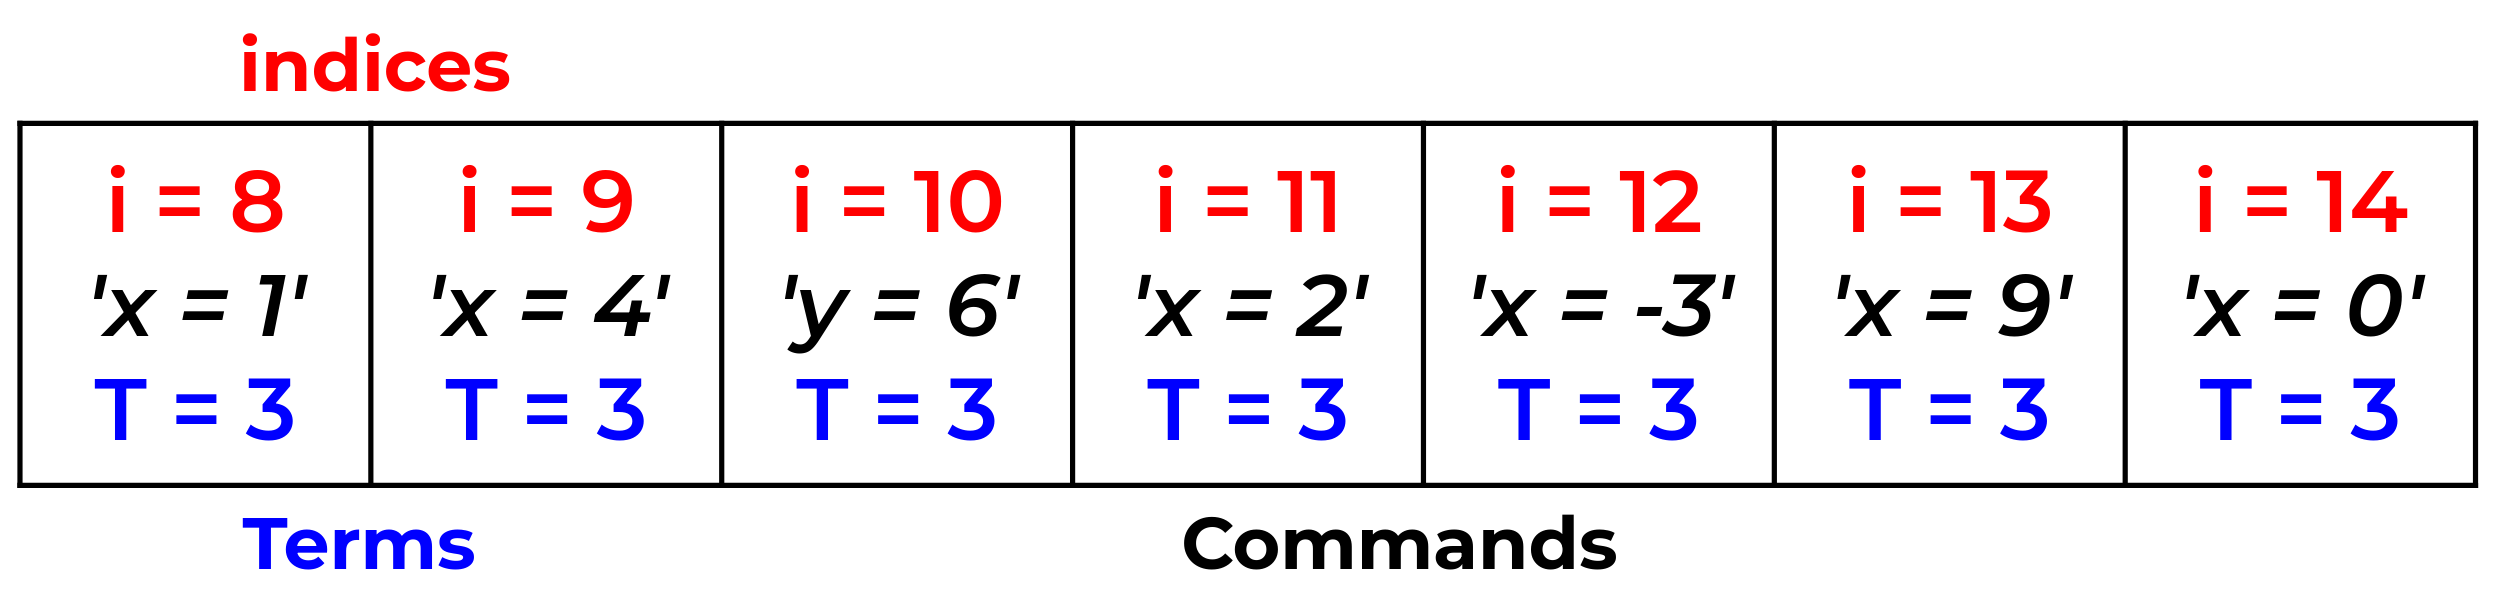
\includegraphics[width=.8\linewidth]{images/logStructure.png}
  
  \caption{Raf's log is fundamentally and array made of entries.}
  \Description{An array, thus a list of consecutive elements, each of wich is an entry with its own index, term and data.}
  \label{fig:logStructure}
\end{figure}

\subsection{Log Replication and Overwriting}

When the leader have some new entries 

\subsubsection{Log Compaction}

\subsection{Leader Election}

\subsection{Cluster Membership Change}

\subsection{Byzantine Raft}